
\documentclass[a4paper,UKenglish,cleveref, autoref, thm-restate]{lipics-v2021}
%This is a template for producing LIPIcs articles. 
%See lipics-v2021-authors-guidelines.pdf for further information.
%for A4 paper format use option "a4paper", for US-letter use option "letterpaper"
%for british hyphenation rules use option "UKenglish", for american hyphenation rules use option "USenglish"
%for section-numbered lemmas etc., use "numberwithinsect"
%for enabling cleveref support, use "cleveref"
%for enabling autoref support, use "autoref"
%for anonymousing the authors (e.g. for double-blind review), add "anonymous"
%for enabling thm-restate support, use "thm-restate"
%for enabling a two-column layout for the author/affilation part (only applicable for > 6 authors), use "authorcolumns"
%for producing a PDF according the PDF/A standard, add "pdfa"

%\pdfoutput=1 %uncomment to ensure pdflatex processing (mandatatory e.g. to submit to arXiv)
%\hideLIPIcs  %uncomment to remove references to LIPIcs series (logo, DOI, ...), e.g. when preparing a pre-final version to be uploaded to arXiv or another public repository

%\graphicspath{{./graphics/}}%helpful if your graphic files are in another directory

\bibliographystyle{plainurl}% the mandatory bibstyle

\title{A Verified Implementation of B$^+$-Trees in Isabelle/HOL} %TODO Please add

%\titlerunning{Dummy short title} %TODO optional, please use if title is longer than one line

\author{Niels Mündler}{Department of Computer Science, ETH Zurich, Switzerland}{n.muendler@tum.de}{https://orcid.org/0000-0003-3851-2557}{}%TODO mandatory, please use full name; only 1 author per \author macro; first two parameters are mandatory, other parameters can be empty. Please provide at least the name of the affiliation and the country. The full address is optional. Use additional curly braces to indicate the correct name splitting when the last name consists of multiple name parts.

\author{Tobias Nipkow}{Department of Informatics, Technical University of Munich, Germany}{nipkow@in.tum.de}{https://orcid.org/0000-0003-0730-515X}{}

\author{Peter Lammich}{Department of Computer Science, The University of Manchester, Great-Britain}{lammich@in.tum.de}{https://orcid.org/0000-0003-3576-0504}{}

\authorrunning{N. Mündler, T. Nipkow and P. Lammich} %TODO mandatory. First: Use abbreviated first/middle names. Second (only in severe cases): Use first author plus 'et al.'

\Copyright{Niels Mündler} %TODO mandatory, please use full first names. LIPIcs license is "CC-BY";  http://creativecommons.org/licenses/by/3.0/

\begin{CCSXML}
    <ccs2012>
       <concept>
           <concept_id>10003752.10003790.10011742</concept_id>
           <concept_desc>Theory of computation~Separation logic</concept_desc>
           <concept_significance>500</concept_significance>
           </concept>
     </ccs2012>
\end{CCSXML}
    
\ccsdesc[500]{Theory of computation~Separation logic}
%TODO mandatory: Please choose ACM 2012 classifications from https://dl.acm.org/ccs/ccs_flat.cfm 

\keywords{Separation Logic, Verification, Refinement} %TODO mandatory; please add comma-separated list of keywords

\category{} %optional, e.g. invited paper

\relatedversion{} %optional, e.g. full version hosted on arXiv, HAL, or other respository/website
%\relatedversiondetails[linktext={opt. text shown instead of the URL}, cite=DBLP:books/mk/GrayR93]{Classification (e.g. Full Version, Extended Version, Previous Version}{URL to related version} %linktext and cite are optional

%\supplement{}%optional, e.g. related research data, source code, ... hosted on a repository like zenodo, figshare, GitHub, ...
%\supplementdetails[linktext={opt. text shown instead of the URL}, cite=DBLP:books/mk/GrayR93, subcategory={Description, Subcategory}, swhid={Software Heritage Identifier}]{General Classification (e.g. Software, Dataset, Model, ...)}{URL to related version} %linktext, cite, and subcategory are optional

%\funding{(Optional) general funding statement \dots}%optional, to capture a funding statement, which applies to all authors. Please enter author specific funding statements as fifth argument of the \author macro.

\acknowledgements{I want to thank \dots}%optional

%\nolinenumbers %uncomment to disable line numbering



%Editor-only macros:: begin (do not touch as author)%%%%%%%%%%%%%%%%%%%%%%%%%%%%%%%%%%
\EventEditors{John Q. Open and Joan R. Access}
\EventNoEds{2}
\EventLongTitle{42nd Conference on Very Important Topics (CVIT 2016)}
\EventShortTitle{CVIT 2016}
\EventAcronym{CVIT}
\EventYear{2016}
\EventDate{December 24--27, 2016}
\EventLocation{Little Whinging, United Kingdom}
\EventLogo{}
\SeriesVolume{42}
\ArticleNo{23}
%%%%%%%%%%%%%%%%%%%%%%%%%%%%%%%%%%%%%%%%%%%%%%%%%%%%%%

\newcommand{\btree}{B$^+$-Tree}
\newcommand{\btrees}{B$^+$-Trees}

\begin{document}

\maketitle

%TODO mandatory: add short abstract of the document
\begin{abstract}
    The abstract will surely become longer at some point.
\end{abstract}

\section{Introduction}
\label{sec:introduction}

This will be the introduction. There will be more text.

\section{\btrees\ and Approach}
\label{sec:approach}

B-trees were first proposed by Bayer in \cite{DBLP:journals/acta/BayerM72},
as a data-structure to efficiently retrieve and manipulate
indexed data stored on storage devices with slow memory access.
They are $n$-ary balanced search trees.
They may be specified as implementing a set interface,
where the indices form the actual content of the set,
the specification that serves as basis in this work.

A commonly implemented variation is the \btree, where the inner nodes
only contain separators to guide the recursive navigation through the tree.
In \btrees, all data is stored in the leaves \cite{DBLP:journals/csur/Comer79}.
Further the leaves are often implemented so as to contain pointers
to the next leaf in order, allowing for efficient range queries.

Nodes are generally thought to be implemented by
containing a number of indices, data corresponding to each index
and a number of children.

\begin{figure}
    \centering
    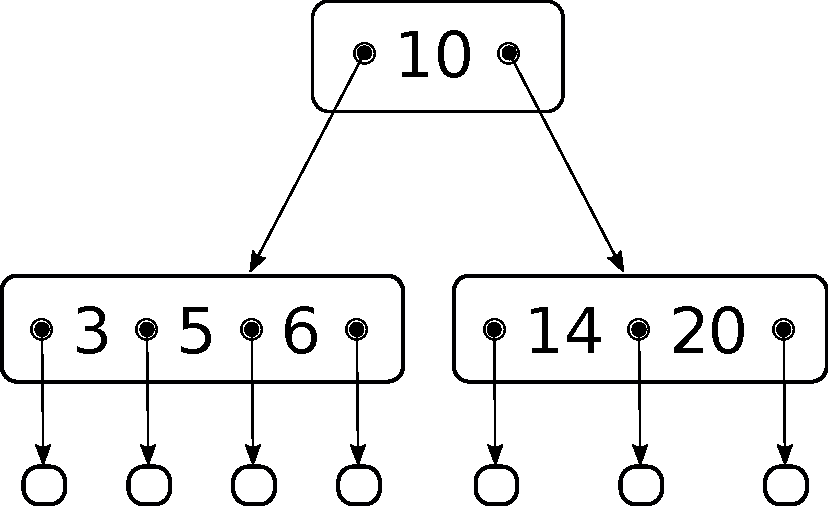
\includegraphics[width=0.5\linewidth]{figures/btree-basic-nopair.pdf}
    \caption[A small example B-Tree]{A small balanced, sorted B-tree of order $2$ and
    height $2$ containing $3$ nodes and $6$ elements.
    In subsequent depictions, leafs will be depicted
    by empty circles.}
    \label{fig:btree-basic-nopair}
\end{figure}


\subsection{Definitions}
\label{sec:data_structure_defs}

Every node contains a list of \textit{keys} (also \textit{separators}, \textit{index elements}), and \textit{subtrees} (\textit{children}),
that represent further B-tree nodes.
The separators and subtrees may be considered interleaved within a node,
such that we can speak of a subtree to the left of a separator and
a subtree to the right of a separator,
where for a separator at index $i$ we mean the subtree in the respective
subtree list at index $i$ and $i+1$ respectively.
Note that this already implies that the list of subtrees is one
longer than the list of separators - we refer to the last subtree
as the \textit{last} or \textit{dangling} subtree.
In the original definition by Bayer \cite{DBLP:journals/acta/BayerM72},
a B-tree with above structure must fulfill the three properties
\textit{balancedness}, \textit{order} and \textit{sortedness}.

\paragraph{Balancedness} \textit{Balancedness} requires
that each path from the root to any leaf has the same length $h$.
In other words, the height of all trees in one level of the tree must be equal,
where the height is the maximum path length to any leaf.
It is only possible to maintain this property
due to the flexible amount of subtrees in each node.

\paragraph{Sortedness} Further the indices must be \textit{sorted} within the tree which means that all indices stored
in the subtree to the left of a separator are smaller than the value of the separator
and all indices in the subtree to the right are greater.
Further all indices within a node should maintain a sorted order,
that is the list of separators in a node must be sorted.

\paragraph{Order} In general terms, the property of \textit{order} ensures a certain minimum and maximum
number of subtrees for each node.
However, as pointed out by Folk and Zoellick \cite{DBLP:books/daglib/0095349_mod},
the property is defined differently in the literature.
For the purpose of this work, the original definition by Bayer
was chosen as most suitable.
A B-tree is of order $k$, if each internal node has at least $k+1$
subtrees and at most $2k+1$.
The root is allowed to have a minimum of 2 subtreess and a maximum of $2k+1$.

An alternative definition proposed by Knuth \cite{DBLP:books/lib/Knuth98a},
is to allow between $\lceil \frac{k}{2} \rceil$ and $k$ children.
However this involves cumbersome \textit{real} arithmetic that unnecessarily complicates
mechanized proofs.
Sticking to the original definition is further supported by the fact that nodes are supposed
to fill memory pages which are usually of even size (usually some power of 2).
An even number of separators and trees plus one dangling last tree maximizes
the usage of such a page.

The same ambiguity exists for the term \textit{Leaf} which we will define consistently with Knuth's definition \cite{DBLP:books/lib/Knuth98a}
to be an empty node, carrying no information,
rather than a node that contains data but no children.
This is close to the usual approach in functional programming,
and will yield more elegant recursive equations for our B-tree operations.
The lowest level of nodes hence contains a list of separators and
list of pointers to leaves as can be seen in \Cref{fig:btree-basic-nopair}.

Note that the B-tree definition is only meaningful for positive $k$.
For the case that $k$ is equal to 0,
all elements of the tree would have exactly one subtree
and no internal elements.
For the root node this even leads to a contradictory state:
It is required to contain at least 1 element or 2 subtrees.
However as it should not have more than $2k+1 = 1$ elements,
this constraint can not be satisfied.
Requiring positive $k$ is consistent with the definitions
in the consulted literature \cite{DBLP:journals/acta/BayerM72,DBLP:journals/csur/Comer79,DBLP:books/daglib/0023376}.

\section{Functional B$^+$-Trees}
\label{sec:functional}

\section{Imperative B$^+$-Trees}
\label{sec:imperative}

\section{Comparison and Conclusion}
\label{sec:conclusion}

\end{document}
